\documentclass[../../memoria.tex]{subfiles}

\begin{document}

\paragraph{}
Otra de las pruebas que se ha realizado contra el sistema es la comunicación en el sentido inverso, es decir, desde la nube hacia los dispositivos. Esta comunicación es importante ya que permite actuar sobre los propios dispositivos sin tener que estar en el mismo lugar físicamente. Esto permitiría actualizar los dispositivos, reiniciarlos, etc.

\paragraph{}
Para la realización de esta prueba se ha decidido implementa un pequeño script en python que sirva como ejemplo, sin implementar un dispositivo o simulador real. El único objetivo de esta prueba es demostrar que es posible esta comunicación. Para ello, se va a hacer uso de las credenciales de uno de los cuatro dispositivos IoT que se despliegan.

\paragraph{}
El script implementará un subscriptor MQTT, que se suscriba a un \textit{IoT Topic} en particular, que se le denominará poc-iot-topic-receptor-1, y se utilizarán las credenciales de uno de los sensores para poder suscribirse a dicho topic. Se ha decidido que el funcionamiento al recibir un mensaje desde el topic sea imprimirlo por pantalla y ejecutar el comando indicado en la máquina donde se lanza el suscriptor. En las siguientes imágenes podemos ver ejemplos de este funcionamiento:

\begin{figure}[H]
    \centering
    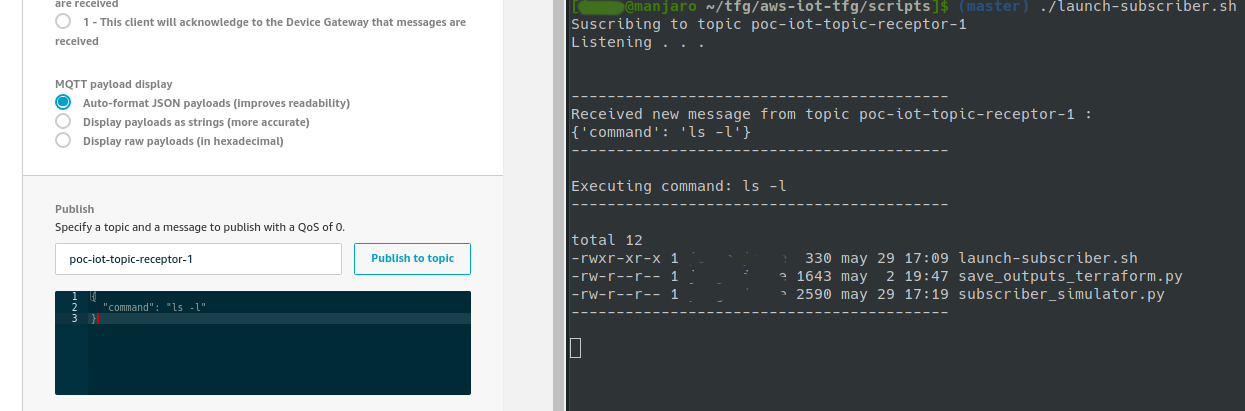
\includegraphics[width=0.7\columnwidth]{pruebaSuscriptor1.png}
    \caption{Prueba 1 de comunicación hacia el dispositivo IoT. Comando ls -l}
    \label{fig:pruebaSuscriptor1}
\end{figure}

\begin{figure}[H]
    \centering
    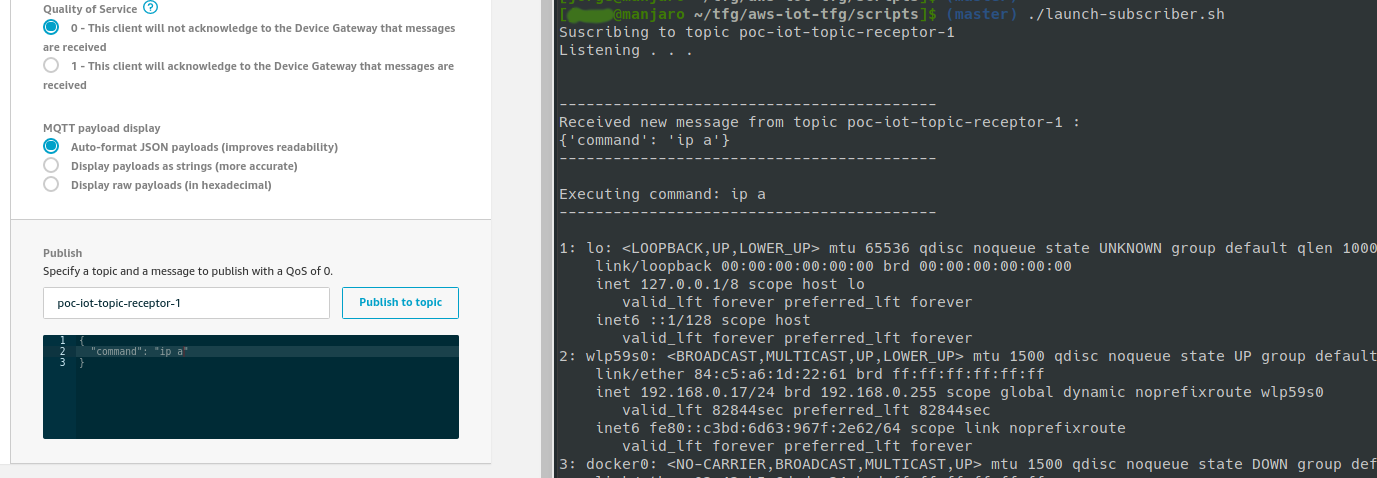
\includegraphics[width=0.7\columnwidth]{pruebaSuscriptor2.png}
    \caption{Prueba 1 de comunicación hacia el dispositivo IoT. Comando ip a}
    \label{fig:pruebaSuscriptor2}
\end{figure}

\begin{figure}[H]
    \centering
    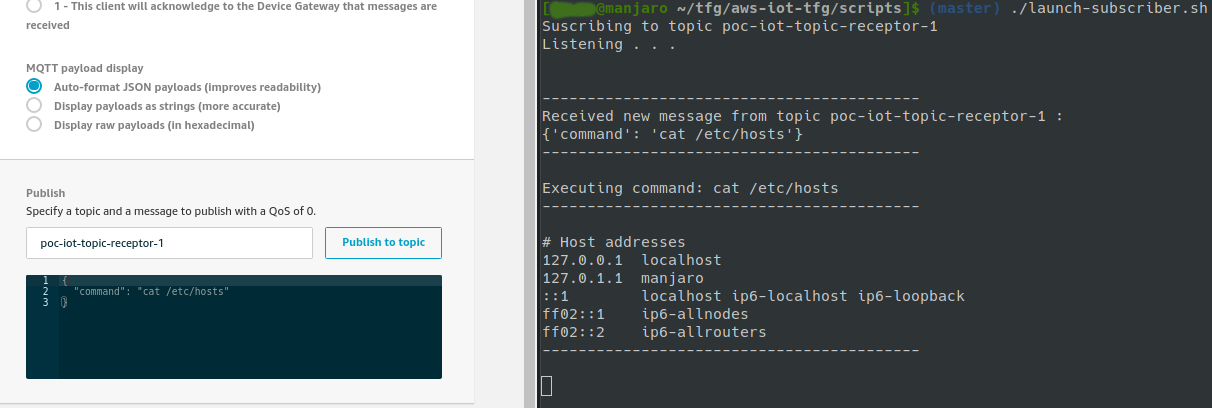
\includegraphics[width=0.7\columnwidth]{pruebaSuscriptor3.png}
    \caption{Prueba 1 de comunicación hacia el dispositivo IoT. Comando cat /etc/hosts}
    \label{fig:pruebaSuscriptor3}
\end{figure}

\paragraph{}
Como puede observarse, se pueden incluso ejecutar comandos de manera remota si el programa suscrito al topic está preparado para ello. De esta manera se puede actualizar el software, cambiar la configuración, etc. sin tener que estar físicamente conectado al dispositivo. En cuanto a la seguridad sobre esto, es necesario asegurar que el \textit{topic} al cual se suscriben los dispositivos tiene restringida la escritura para que no haya compromisos de seguridad.

\paragraph{}
Con esta pequeña prueba se demuestra lo simple que sería poder actuar sobre los dispositivos IoT utilizando el mismo protocolo utilizado para publicar los mensajes hacia la nube.
\end{document}
